\documentclass[slidestop,compress,mathserif]{beamer}
\usepackage[brazil]{babel}
\usecolortheme{sidebartab}
\usepackage{verbatim} % http://devdaily.com/blog/post/latex/multi-line-comments-in-latex-begin-123-comment-125-verbatim
\usepackage[utf8]{inputenc}

\usepackage{graphicx}
\DeclareGraphicsExtensions{.jpg,.pdf,.mps,.png,.gif,.eps}
\graphicspath{{../images/}} %define diretório de imagens

\usepackage{hyperref}
\usepackage{url}
\usetheme{Warsaw}
%\usecolortheme{crane}
\title{Defesa de Mestrado:\\Arquitetura orientada a serviços para comércio eletrônico no Sistema Brasileiro de TV Digital}
\author{Manoel Campos da Silva Filho\\Orientador: Prof. Dr. Paulo Roberto de Lira Gondim}
\institute{Programa de Pós-Graduação em Engenharia Elétrica\\Universidade de Brasília}
\logo{
\includegraphics[scale=.2]{unb.png}}


\setbeamertemplate{footline}[frame number]
%apenas se for usar o compilador xetex
%\usepackage{fontspec}
%\usepackage{xltxtra,xunicode}
%\defaultfontfeatures{Mapping=tex-text}
%\setromanfont[Mapping=tex-text]{Times New Roman}
%\setsansfont[Scale=MatchLowercase,Mapping=tex-text]{Gill Sans}
%\setmonofont[Scale=MatchLowercase]{Andale Mono}
\usepackage{listings}
\lstset{numbers=left,
language=TeX,
stepnumber=1,
firstnumber=1,
numberstyle=\tiny,
extendedchars=true,
breaklines=true,
frame=TB,
basicstyle=\footnotesize,
stringstyle=\ttfamily,
showstringspaces=false
backgroundcolor=\color{gray}
}

\renewcommand{\lstlistingname}{Código Fonte}
\renewcommand{\lstlistlistingname}{Lista de Códigos Fonte}

\begin{document}


\frame{\titlepage} 

\begin{comment}
\begin{frame}[allowframebreaks] %Permite que o roteiro seja quebrado em vários slides
  \frametitle{Roteiro}
  \setcounter{tocdepth}{1} %Exibe apenas os elementos de primeiro nível no sumário
  \tableofcontents
\end{frame}
\end{comment}

\frame{\frametitle{Roteiro}
  \setcounter{tocdepth}{1} %Exibe apenas os elementos de primeiro nível no sumário
  \tableofcontents
}


\begin{comment}
\section[Intro]{Introdução} 
\frame{\frametitle{Introdução} 
\begin{itemize}
	\item Aumento do uso de sistemas de compras via Internet
	\item Vários casos de sucesso de lojas virtuais no Brasil e no mundo
	\item Fatores de Sucesso das Lojas Virtuais
  \begin{itemize}
	  \item Comodidade; possibilidade de melhor avaliação dos produtos
	  \item Atendimento especializado com uso de sistemas de informação
	  \item Sistemas de recomendação de produtos
	\end{itemize}	
	\item Pesquisa Nacional TIC Domicílios\cite{tic2009}: 2008 para 2009
  \begin{itemize}
	  \item aumento de 8\% na consulta a preços de produtos/serviços na \textit{Web}
	  \item consultas (de 44\% para 52\%)
	  \item crescimento nas compras \textit{on line} de 3\% (de 16\% p/ 19\%)
	  \item 32\% dos domicílios tinham computador (contra 25\% em 2008)
	  \item 25\% tinham acesso à \textit{Internet} (contra 18\% em 2008)
	\end{itemize}	
\end{itemize}
}

\frame{\frametitle{Introdução} 
\begin{itemize}
	\item Apresentação da Arquitetura Proposta
  \begin{itemize}
	  \item Arquitetura para prover comércio eletrônico no SBTVD
	  \item Baseada em serviços web e arquitetura SOA
	  \item Base para a construção de aplicações de T-Commerce
    \begin{itemize}
	    \item Compras
	    \item Rastreamento de Encomendas
	    \item Notícias RSS
	  \end{itemize}	
	  
	  \item Aplicativos baseados em templates e temas: Framework LuaOnTV 2.0
	  \item Integração Web/TV com HTTP e SOAP: Framework de Comunicação de Dados
	\end{itemize}		
\end{itemize}
}
\end{comment}

\section[ObjGeral]{Objetivo Geral}
\frame{\frametitle{Objetivo Geral}
\begin{itemize}
	\item Propor e desenvolver uma arquitetura orientada a serviços,
  por meio de \textit{Web Services} SOAP, para provimento de comércio eletrônico
  pela TV Digital, favorecendo a convergência \textit{Web}-TV. 
\end{itemize}
}

\section[ObjEspec]{Objetivos Específicos}
\frame{\frametitle{Objetivos Específicos}
\begin{itemize}
  \item Propor uma arquitetura baseada em serviços \textit{Web} para \textit{T-Commerce};
  
	\item implementar um \textit{framework} para comunicação de dados (HTTP e SOAP);
	
  \item \textit{framework} de comunicação de dados para desenvolvimento de aplicações
  (RSS, Rastreador, Twitter, etc);
	
	\item estender o \textit{framework} LuaOnTV\cite{junior2009luacomp}: temas, suporte a 
	múltiplas resoluções de tela (TV's e celulares);
	
	\item modelo de desenvolvimento de aplicações para TVD com uso de \textit{templates};
  	
	\item montar uma distribuição Linux.
\end{itemize}
}

\section[Just]{Justificativa}
\frame{\frametitle{Justificativa}
\begin{itemize}
	\item Poucos casos de T-Commerce no Brasil (ver \cite{extra-vendas-tvd}) e no mundo;
	\item casos brasileiros não permitem finalizar a compra pela TV;
	\item sucesso do E-Commerce no Brasil e no mundo;
	\item cerca de 96\% dos lares brasileiros têm TV\cite{ibge-pnad} (switch-off analógico em 2016);
	\item falta de uma arquitetura de T-Commerce para o SBTVD;
	\item integração entre Web e TV com uso de HTTP e SOAP.
\end{itemize}
}

\begin{comment}
\subsection{Metodologia}
\frame{\frametitle{Metodologia}
\begin{itemize}
	\item Levantamento bibliográfico
	\item Projeto, análise e desenvolvimento: processo de desenvolvimento em cascata com componentização
  \begin{itemize}
	  \item requisitos bem definidos (assumiu-se o papel do usuário na especificação)
	  \item componentes reutilizáveis (Web Services)
  \end{itemize}
  \item Etapas seguidas do processo em  cascata:
  \begin{itemize}
	  \item Especificação de requisitos;
	  \item Projeto OO, UML, Ferramentas CASE;
	  \item Implementação;
	  \item Testes de interoperabilidade/integração.
  \end{itemize}
  \item Requisitos levantados com base em Web Sites de E-Commerce
\end{itemize}
}


\section[Revisão]{Revisão Bibliográfica}
\frame{\frametitle{Revisão Bibliográfica}
\vspace{3cm}
\begin{center}\large{Revisão Bibliográfica}\end{center}
}

\subsection{Comércio Eletrônico}
\frame{\frametitle{Comércio Eletrônico}
  \begin{itemize}
		\item Segundo \cite{veijalainen2006transaction}:
    \begin{quote} 
    "uma transação eletrônica
    é uma venda ou compra de produtos ou serviços, entre empresas, familiares, indivíduos, governos e outras organizações
    públicas ou privadas, conduzidas por redes mediadas por computador."
    \end{quote}
    \item \textit{Eletronic Data Interchange}
    \item Advento de padrões XML
    \item Comércio Móvel: transações feitas meio de dispositivos e redes móveis\cite{veijalainen2006transaction}.
    \item T-Commerce
	\end{itemize}	
}

\subsection[SBTVD]{Sistema Brasileiro de TV Digital (SBTVD)}
\frame{\frametitle{Sistema Brasileiro de TV Digital (SBTVD)}
  \begin{itemize}
		\item Baseado no padrão Japonês ISDB-T\footnote{Integrated Services Digital Broadcasting Terrestrial}
		\item Conhecido internacionalmente como ISDB-TB
		\item Instituído por Decreto o Fórum SBTVD
    \item Usa o padrão Ginga como \textit{middleware}
    \begin{itemize}
  		\item abstração de hardware e SO; controle do ciclo de vida das apps; API's e EPG
  		\item Ginga-J (Java): obrigatório apenas em receptores fixos
  		\item Ginga-NCL (NCL e Lua): receptores fixos, móveis e portáteis
  		\item Recomendações: ITU-T J.200 (Ginga), ITU-T J.201 (Ginga-NCL), ITU-T J.202 (Ginga-J),  H.761 (Ginga-NCL para IPTV)
  	\end{itemize}	
  \end{itemize}	
}

\subsection{Web Services}
\frame{\frametitle{A Tecnologia de Web Services}
  \begin{itemize}
		\item Necessidade de integração de aplicações heterogêneas
		\item Aplicações fazendo acesso a BD's via Web (\textit{firewall friendly})
		\item Aplicações distribuídas na Web
		\item Um sistema distribuído traz benefícios como: permitir a heterogeneidade de componentes,
possibilitar a escalabilidade, ser tolerante a falhas, dentre outros\cite{coulouris2007sisdist}
    \item Maior tecnologia para publicação de serviços na \textit{Web}; adoção em integração de aplicações, computação distribuída de larga escala e B2B\cite{kopecky2008semantic}
    \item Desenvolvimento baseado em componentes, acessíveis por meio da \textit{Internet}\cite{sommerville2011soft}
    \item Baseado em padrões XML abertos: SOAP, WSDL, UDDI\footnote{Universal Description, Discovery and Integration}
    \item Arquitetura Orientada a Serviços
	\end{itemize}	
}
\end{comment}


\section[Arq]{Arquitetura de T-Commerce}
\frame{\frametitle{Arquitetura de T-Commerce}
\begin{itemize}
	\item Arquitetura distribuída, baseada em componentes reutilizáveis, os \textit{Web Services};
	\item baseada em SOA; diferentes provedores de serviços;
	\item provedores heterogêneos;
	\item utiliza uma implementação de um \textit{framework} de comunicação (HTTP e SOAP);
	\item SOAP x REST.
\end{itemize}
}

\subsection[Requisitos]{Requisitos da Arquitetura}
\frame{\frametitle{Requisitos da Arquitetura}
\begin{center}
  \scriptsize{
	\begin{tabular}{|p{9.5cm}|c|c|}
	  \hline 
		\textbf{Requisito}& \textbf{F} & \textbf{NF} \\
		\hline 
		T-01) Estar preparada para adaptação em qualquer 
equipamento com qualquer implementação do \textit{middleware} Ginga, seja para dispositivos fixos (como conversores
digitais e TV's com conversores integrados), móveis (como \textit{Notebooks}) ou portáteis (como telefones celulares). & & x \\
		\hline 
		T-02) Utilizar, preferencialmente, serviços gratuitos da \textit{Web}. & & x \\
		\hline 
		T-03) Facilitar o desenvolvimento de aplicações interativas para o SBTVD, inclusive
		com relação ao tratamento de recursos de interface gráfica. & x & \\
		\hline 
		T-04) Tornar transparente para a aplicação de TVD os provedores de serviços utilizados,
		permitindo a substituição por outros apenas estendendo-se classes na aplicação cliente
		e implementando a comunicação SOAP/HTTP com os provedores desejados. & x &  \\
		\hline 
		T-05) Facilitar a extensão e a manutenção das aplicações com uso de orientação a objetos e padrões de projetos. & x &\\
		\hline 		
		T-06) Fazer interoperação com serviços de forma amigável a \textit{firewalls}. &  & x \\
		\hline 
		T-07) Integrar diferentes serviços para compor as funcionalidades a serem disponibilizadas aos usuários das aplicações de TVDi. & x &\\
		\hline 		
	\end{tabular}
	}
	\label{tab:requisitos-arquitetura}
\end{center}

}

\subsection[Apresentação]{Apresentação Geral da Arquitetura}
\frame{\frametitle{Apresentação Geral da Arquitetura} 
  \begin{center}
	  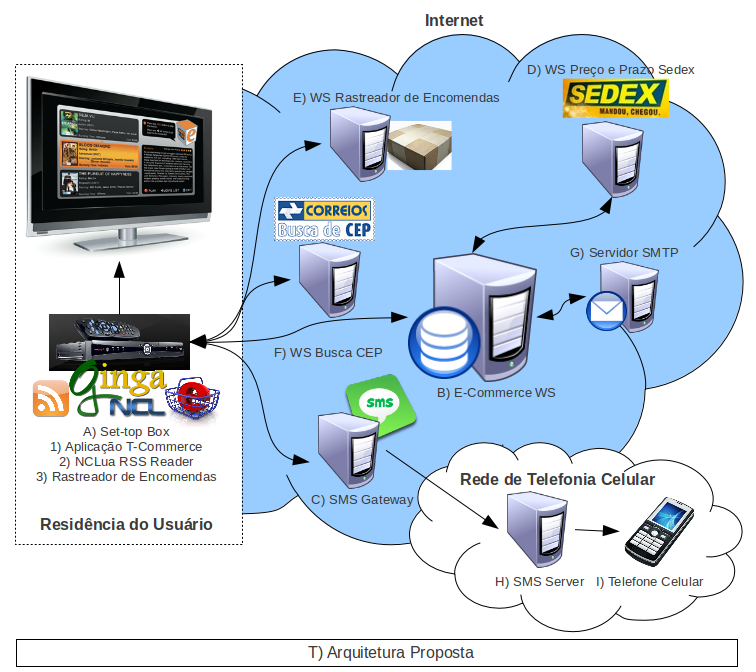
\includegraphics[width=0.8\textwidth]{TCommerce-Arquitetura.png}
	  \label{fig:arquitetura-tcommerce}
  \end{center}  
}

\subsection[UC]{Casos de Uso: Funcionalidades providas a desenvolvedores}
\frame{\frametitle{Casos de Uso: Funcionalidades providas a desenvolvedores}
\begin{center}
	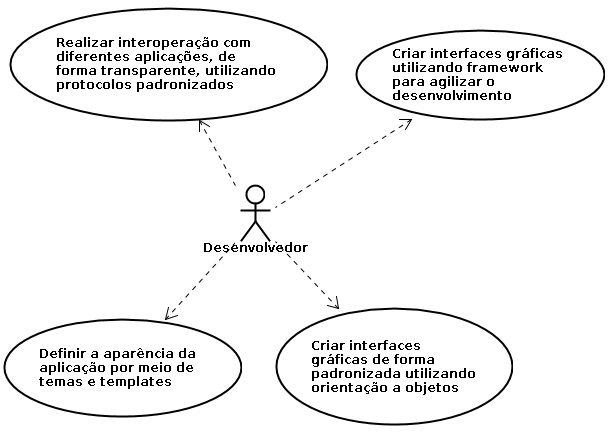
\includegraphics[width=0.8\textwidth]{TCommerce-Diagrama-Casos-de-Uso-Desenvolvedor.png}
	\label{fig:use-case-developer}
\end{center}
}

\frame{\frametitle{Casos de Uso: Funcionalidades providas aos usuários}
\begin{center}
	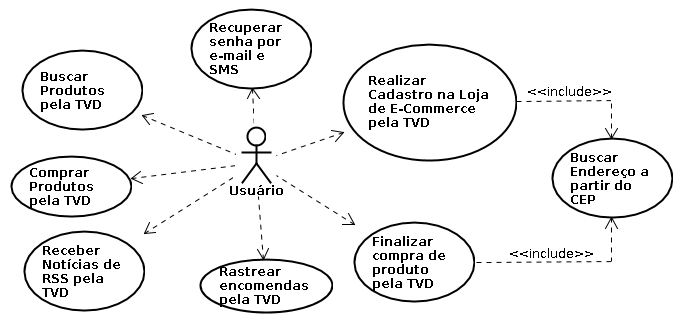
\includegraphics[width=0.8\textwidth]{TCommerce-Diagrama-Casos-de-Uso-Usuario.png}
	\label{fig:use-case-usuario}
\end{center}
}


\subsection[CT]{Tecnologias Core da Arquitetura}
\frame{\frametitle{Tecnologias Core da Arquitetura}
\begin{center}
	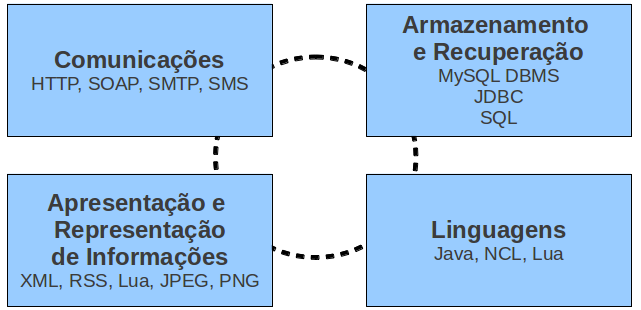
\includegraphics[width=0.8\textwidth]{TCommerce-Arquitetura-CoreTech.png}
	\label{fig:tcommerce-core-tech}
\end{center}
}

\subsection[SW]{Descrição dos Componentes de Software da Arquitetura}
\frame{\frametitle{Descrição dos Componentes de Software da Arquitetura}
Requisitos da aplicação de T-Commerce:
\begin{center}
\scriptsize{
	\begin{tabular}{|p{9.5cm}|c|c|}
		\hline 
  		\textbf{Requisito} & \textbf{F} & \textbf{NF} \\
		\hline
	  	A.1-01) Permitir a exibição de produtos em destaque ao iniciar a aplicação &  X &    \\
		\hline
		  A.1-02) Realizar a busca de produtos pelo título parcial &  X &    \\
		\hline
		  A.1-03) Adicionar produtos ao carrinho de compras &  X &    \\
		\hline
		  A.1-04) Remover produtos do carrinho de compras &  X &    \\
		\hline
		  A.1-05) Cadastrar vários endereços, permitindo ao usuário escolher um endereço
		   de entrega a partir da lista de endereços cadastrados &  X &    \\
		\hline
		  A.1-06) Permitir múltiplas formas de pagamento, possibilitando ao usuário selecionar uma das formas
		   suportadas &  X &    \\
		\hline
		  A.1-07) Cadastrar usuário &  X &    \\
		\hline
		  A.1-08) Realizar login de usuário utilizando \textit{e-mail} ou CPF &  X &    \\
		\hline
		  A.1-09) Buscar endereço a partir do CEP &  X &    \\
		\hline
		  A.1-10) Recuperar senha por \textit{e-mail} e SMS &  X &    \\
		\hline
		  A.1-11) Rastrear automatizadamente encomendas postadas pelos Correios,
		   exibindo ao usuário informações sempre que a situação
		   da encomenda mudar &  X &    \\
		\hline
		  A.1-12) Exibir preço e prazo de entrega, baseado em \textit{Web Services} dos Correios &  X &    \\
		\hline
	\end{tabular}
}	
\end{center}
}

\frame{\frametitle{Descrição dos Componentes de Software da Arquitetura}
Requisitos da aplicação de T-Commerce (continuação): 
\begin{center}
\scriptsize{
	\begin{tabular}{|p{9.5cm}|c|c|}
		\hline 
  		\textbf{Requisito} & \textbf{F} & \textbf{NF} \\	
		\hline
		  A.1-13) Realizar processo de compra em etapas, permitindo que o usuário volte a uma etapa anterior,
		   antes de finalizar a compra, para alterar algum dado (como mudar a forma de pagamento) &  X &    \\
		\hline
		  A.1-14) Utilizar botões coloridos do controle remoto para o acionamento da maioria
		   das funções da aplicação &  X &    \\
		\hline
		  A.1-15) Processar grande parte das regras de negócio nos servidores \textit{Web} que integram a arquitetura,
		   desonerando o conversor digital da maior parte da carga de processamento, considerando
		   que o mesmo é um dispositivo de recursos restritos &   & X   \\
		\hline
		  A.1-16) Armazenar dos dados do carrinho de compras em memória RAM até a finalização da compra,
		   quando estes dados são enviados ao \textit{Web Service} para registro da mesma &   & X   \\
		\hline
		  A.1-17) Carregar dinâmicamente a lista de produtos a partir do \textit{Web Service} &   & X   \\
		\hline
		  A.1-18) Permitir a exibição de comunicados, ofertas de produtos e promoções & X &    \\
		\hline
	\end{tabular}
}	
\end{center}
}

\begin{comment}
\frame{\frametitle{Descrição dos Componentes de Software da Arquitetura}
Screenshot da aplicação de T-Commerce em execução (LuaOnTV + NCLua SOAP)
\begin{center}
	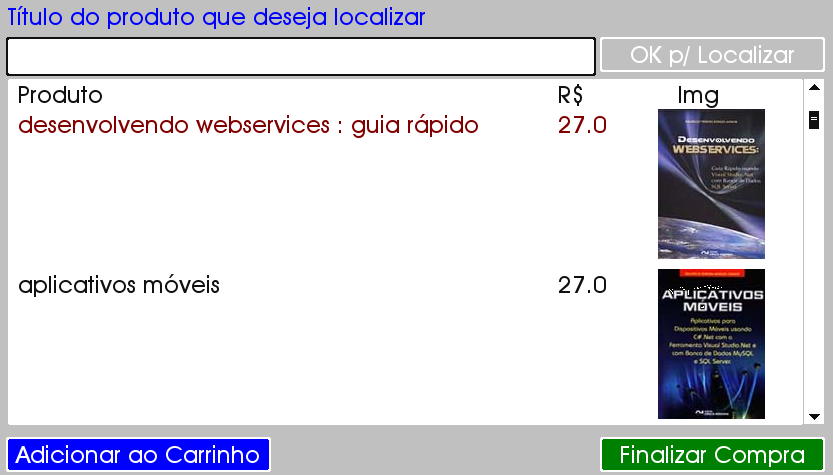
\includegraphics[width=1.00\textwidth]{CommerceApp/TCommerce-App-Destaques.png}
	\label{fig:tcommerce-app-destaques}
\end{center}
}

\frame{\frametitle{Processo de compra (Diagrama de Sequência)}
\begin{center}
	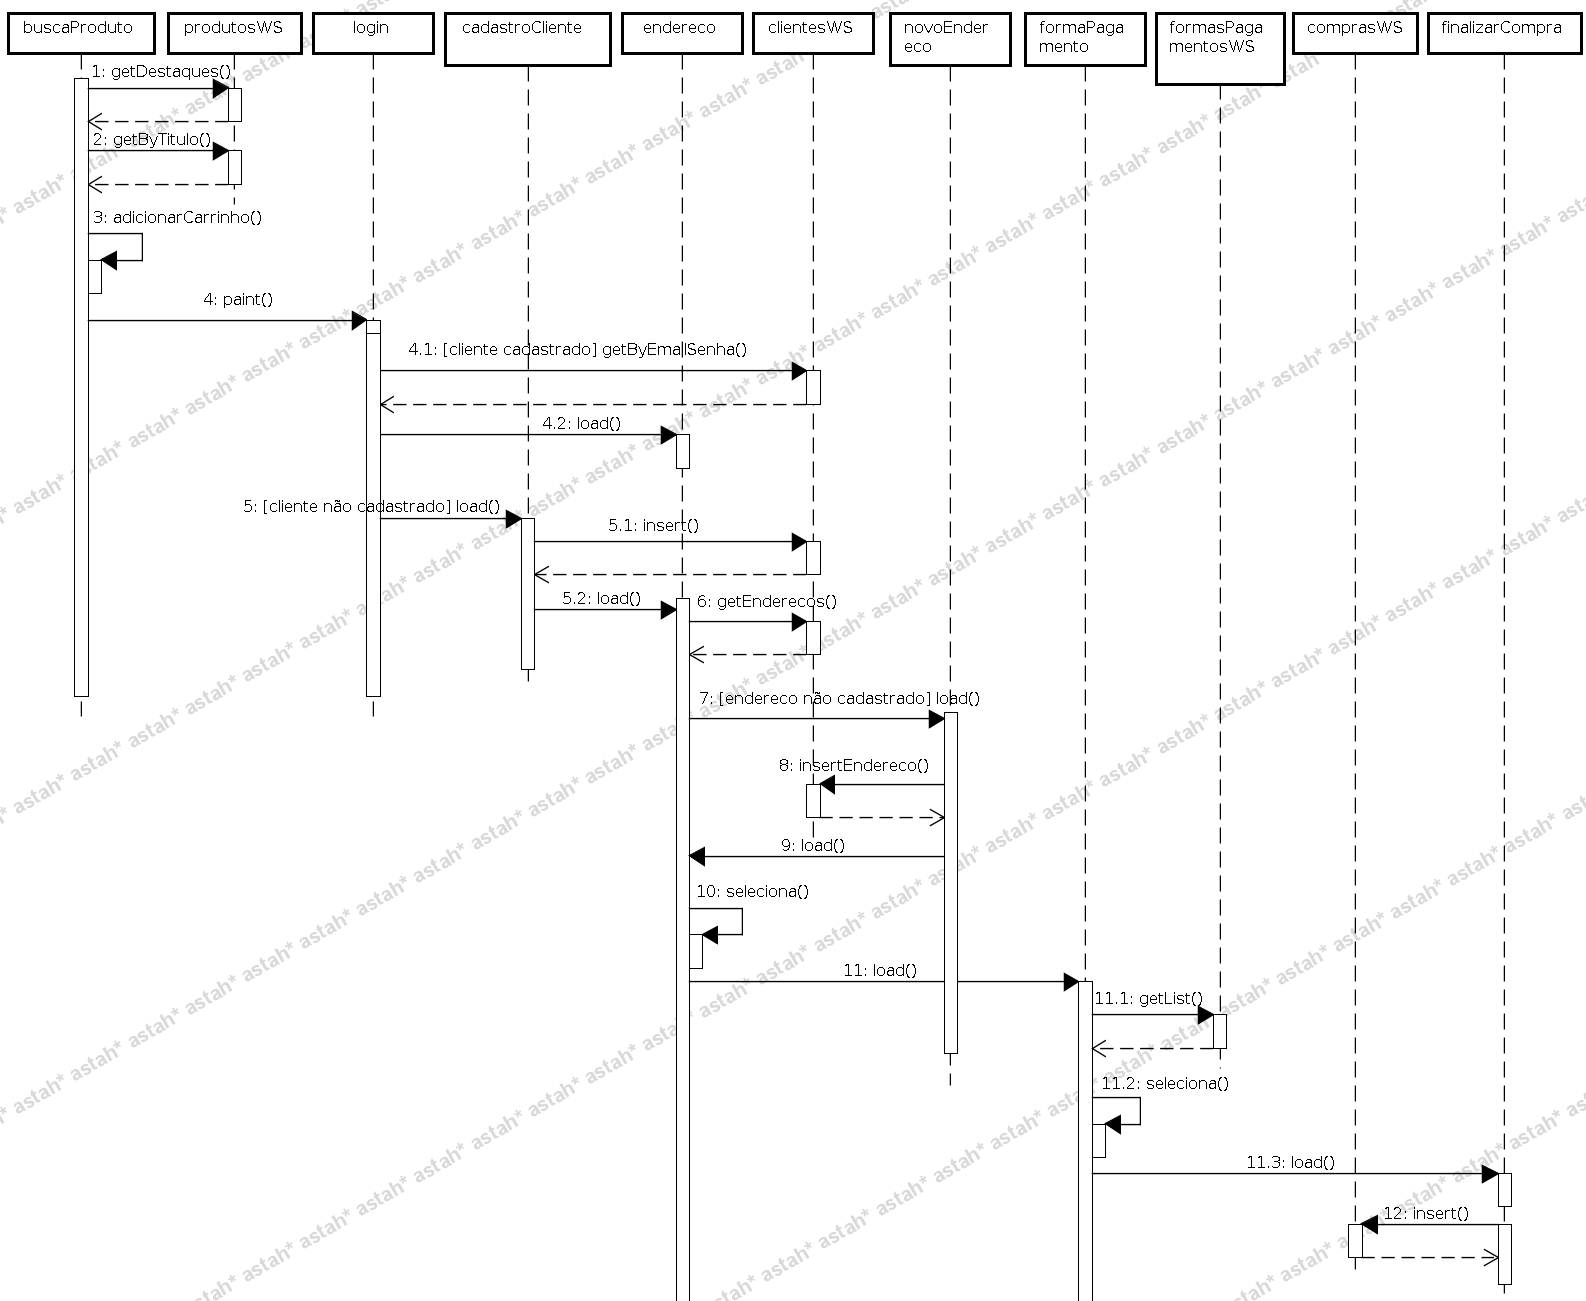
\includegraphics[width=0.9\textwidth]{TCommerce-Diagrama-Sequencia-Compra.png}
	\label{fig:tcommerce-app-diagrama-seq-compra}
\end{center}
}

\frame{\frametitle{Descrição dos Componentes de Software da Arquitetura}
NCLua RSS Reader
\begin{center}
	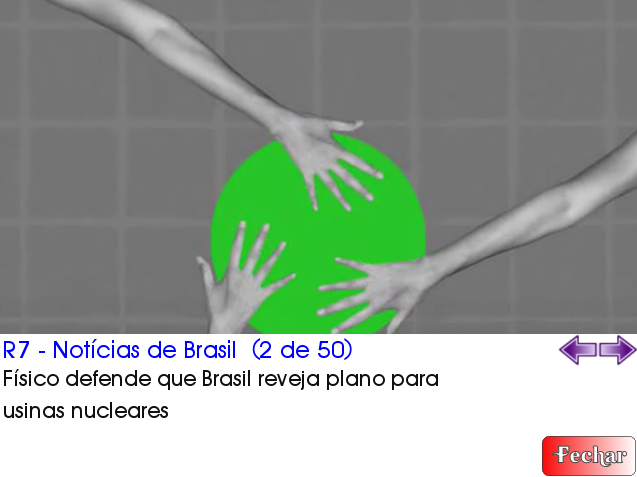
\includegraphics[width=0.8\textwidth]{nclua-rss-reader.png}
	\label{fig:ncluarssreader}
\end{center}
}

\frame{\frametitle{Descrição dos Componentes de Software da Arquitetura}
Rastreador de Encomendas para TVD
\begin{center}
	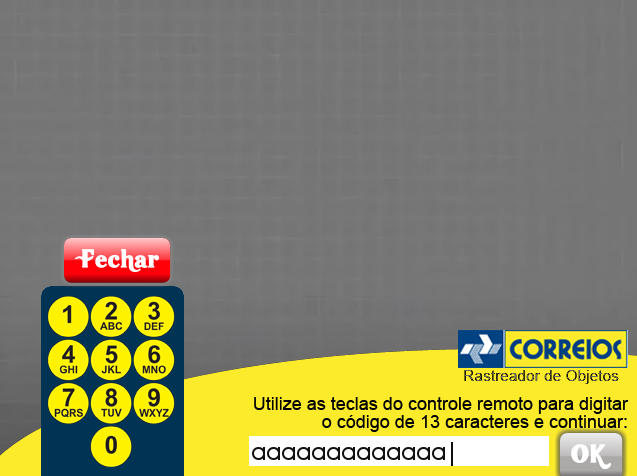
\includegraphics[width=0.8\textwidth]{rastreador/rastreador1.png}
	\label{fig:rastreador-encomendas-tvd1}
\end{center}
}

\frame{\frametitle{Descrição dos Componentes de Software da Arquitetura}
Rastreador de Encomendas para TVD
\begin{center}
	
\includegraphics[width=0.8\textwidth]{rastreador/rastreador2.png}
	\label{fig:rastreador-encomendas-tvd2}
\end{center}
}
\end{comment}

\frame{\frametitle{Descrição dos Componentes de Software da Arquitetura}
E-Commerce WS (Diagrama de Classes Principal)
\begin{center}
	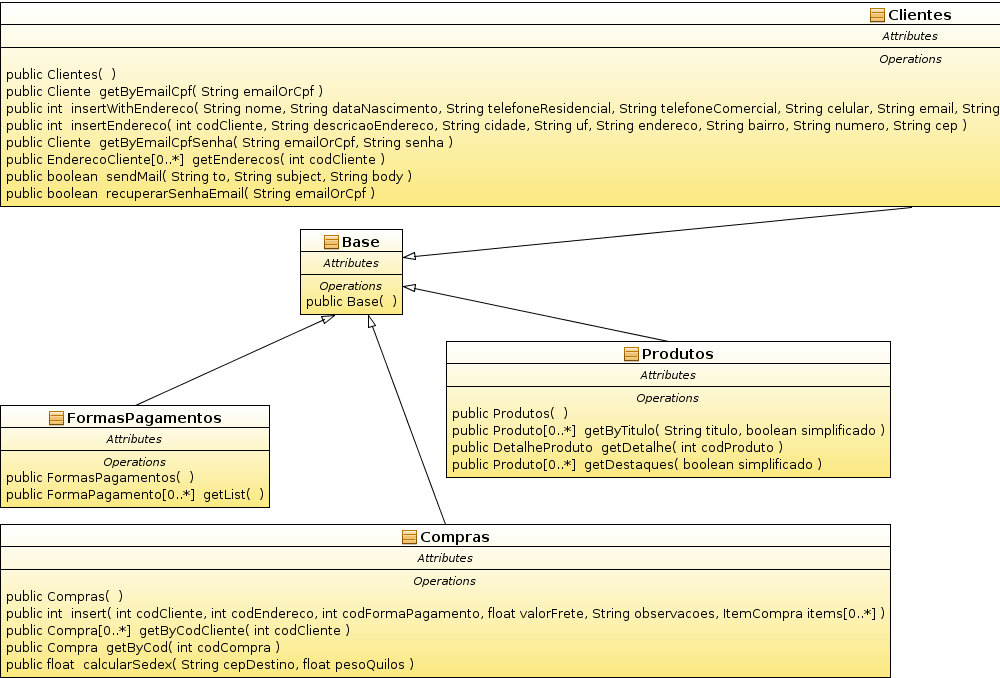
\includegraphics[width=1.00\textwidth]{TCommerce-ClassDiagramServices.png}
	\label{fig:tcommerce-ws}
\end{center}
}

\begin{comment}
\frame{\frametitle{E-Commerce WS (Diagrama de Classes Internas)}
\begin{center}
	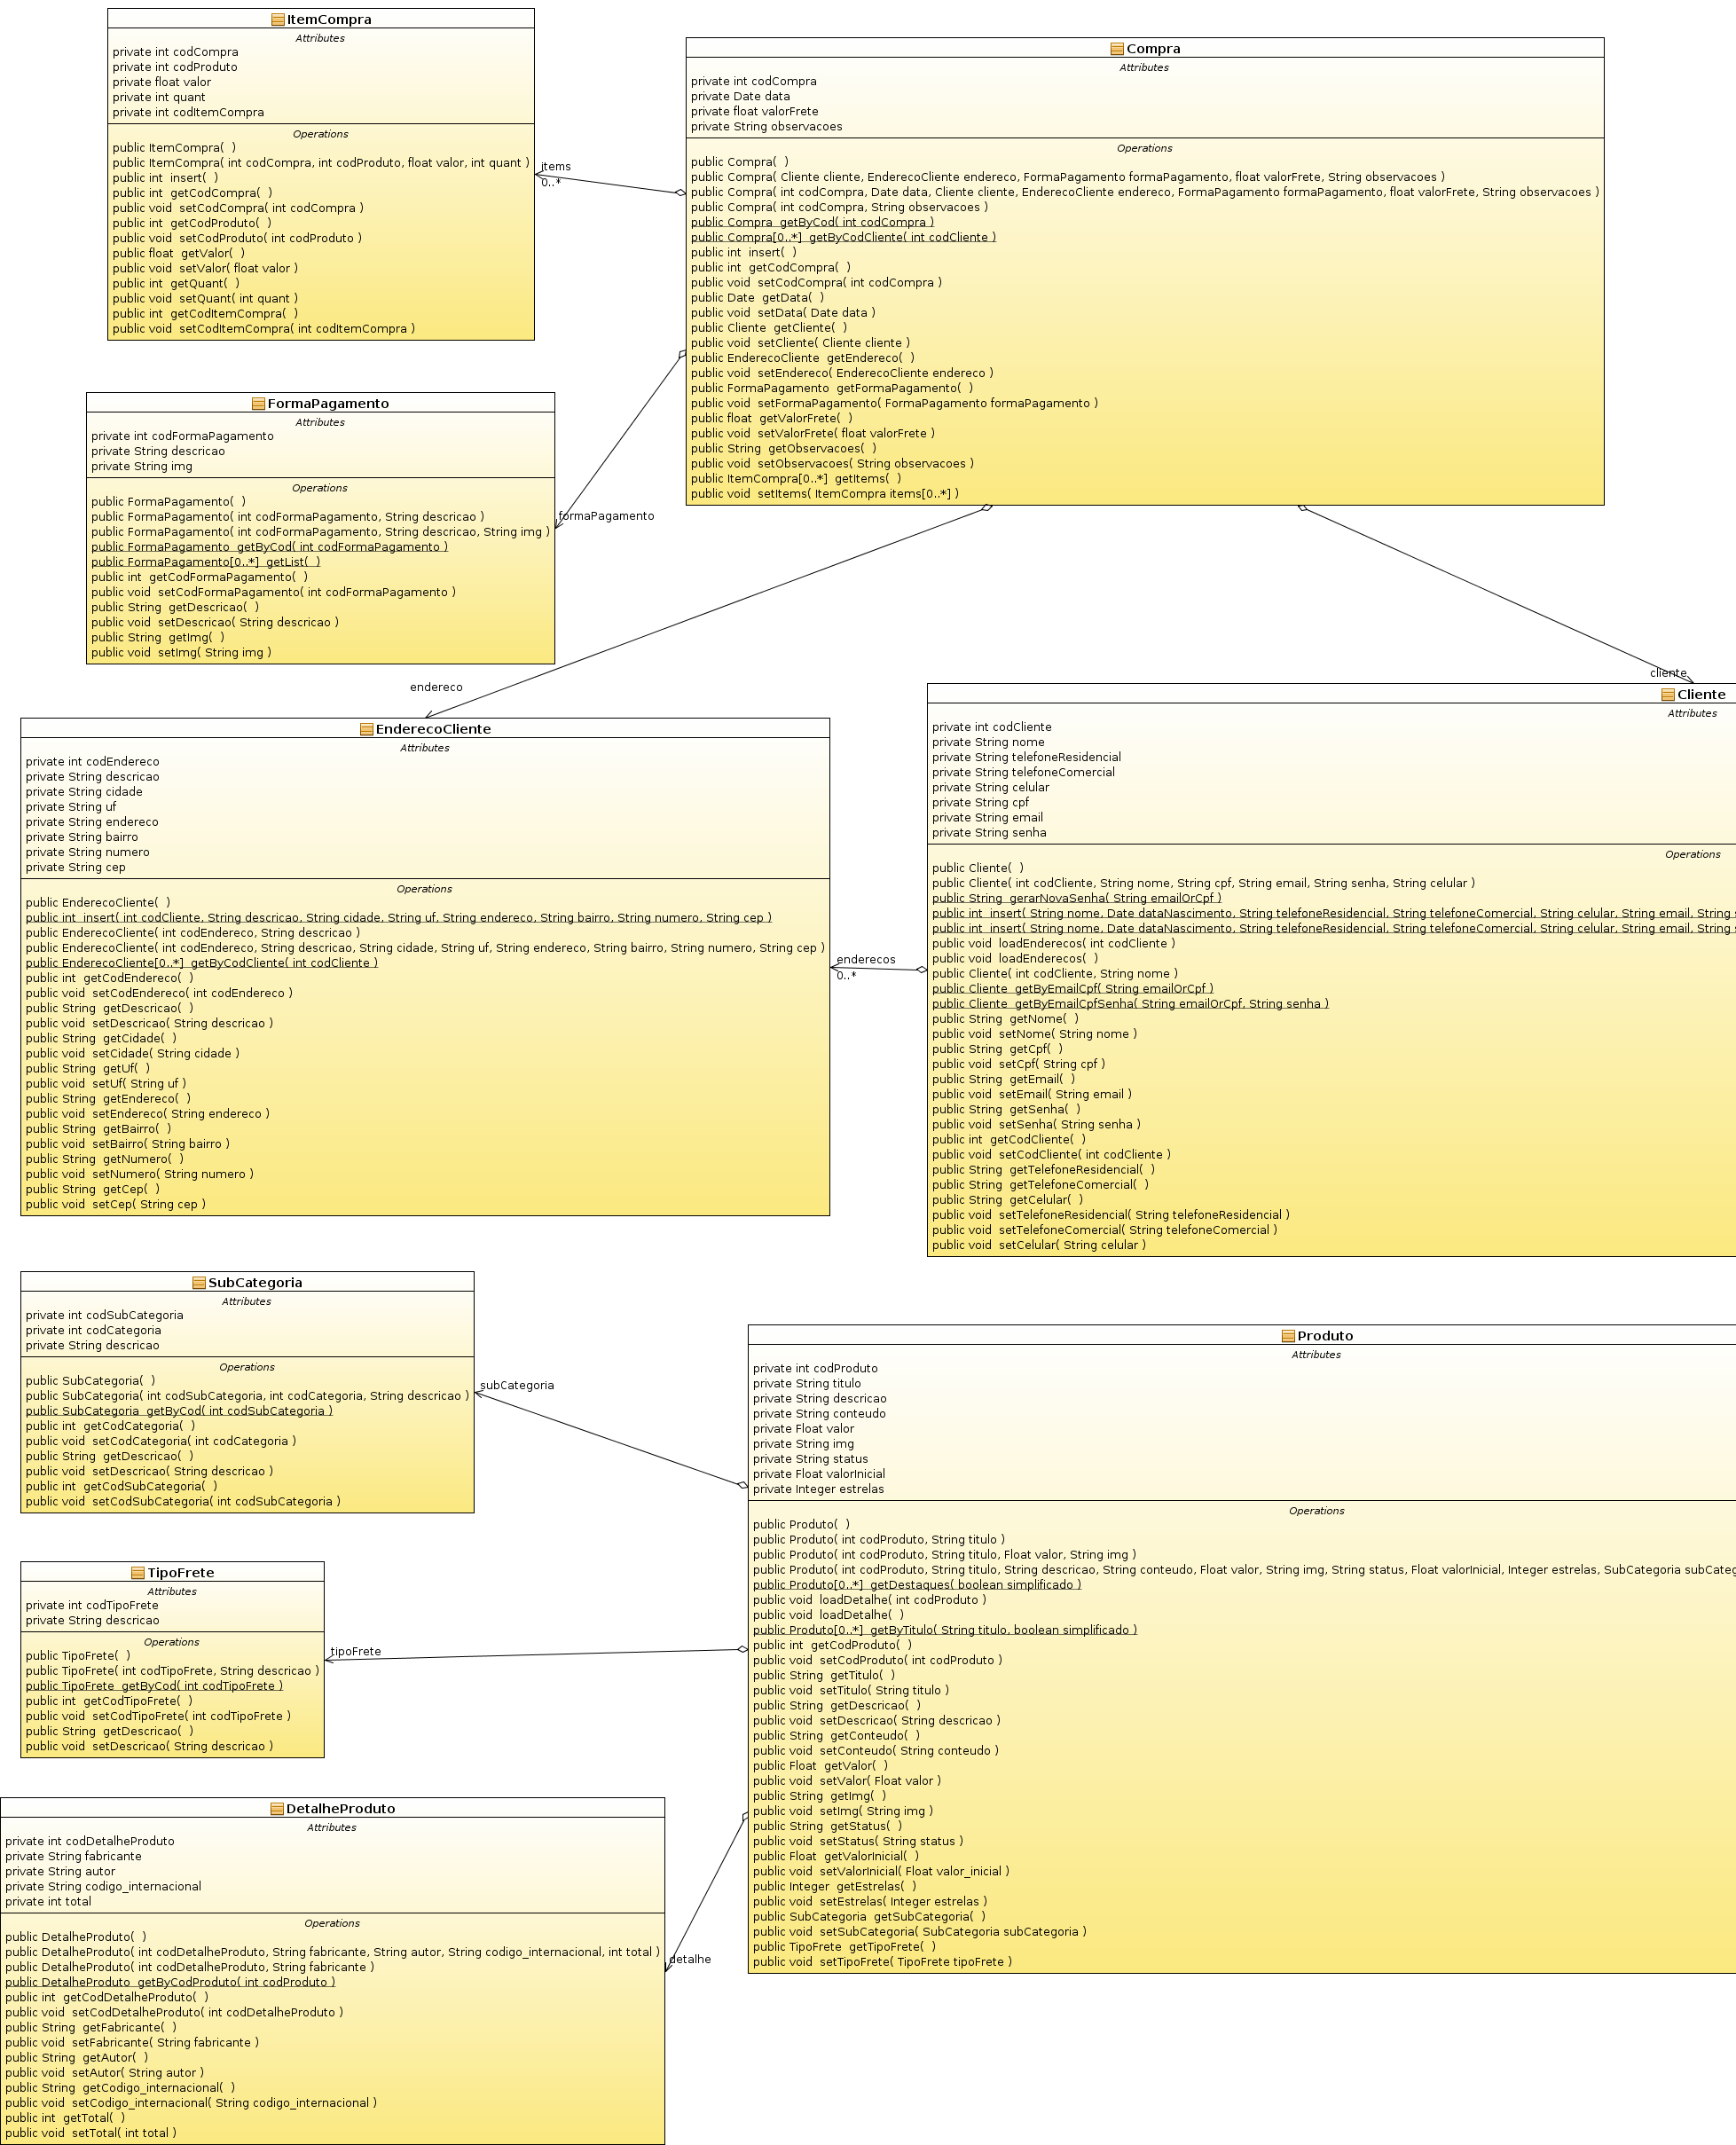
\includegraphics[scale=0.12]{TCommerce-ClassDiagramModel.png}
	\label{fig:tcommerce-ws-classes}
\end{center}
}
\end{comment}


\subsection[Deploy]{Diagrama de Distribuição/Implantação da Arquitetura}
\frame{\frametitle{Diagrama de Distribuição/Implantação da Arquitetura}
\begin{center}
	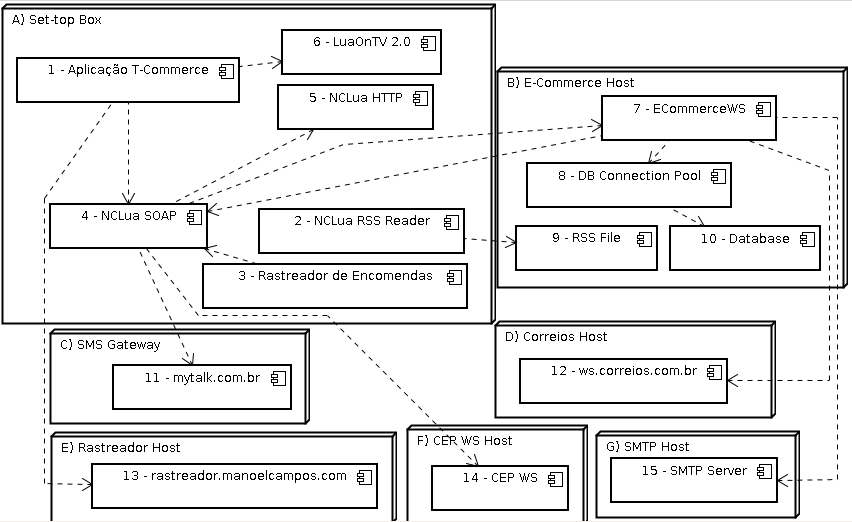
\includegraphics[width=1.00\textwidth]{TCommerce-Diagrama-Distribuicao.png}
	\label{fig:diag-distribuicao}
\end{center}
}

\subsection[Distro]{Distribuição Linux para Desenvolvimento de Aplicações} 
\frame{\frametitle{Distribuição Linux para Desenvolvimento de Aplicações}
\begin{itemize}
	\item Ambiente de desenvolvimento e teste de Aplicações de TVDi em NCL/Lua;
	\item inclui Ginga-NCL nativamente instalado;
	\item ganho de desempenho com a instalação nativa do Ginga-NCL;
	\item baseada em GNU/Linux Ubuntu 10.10;
	\item pode ser usado como sistema operacional padrão para as atividades do dia-a-dia e de desenvolvimento.
\end{itemize}
}

\begin{comment}
\section{LuaOnTV} 
\frame{\frametitle{Framework LuaOnTV\cite{junior2009luacomp}}
\begin{itemize}
	\item Criação de interfaces gráficas em NCL/Lua para o SBTVD;
	\item Delimitação do Problema:
	\begin{itemize}
		\item NCL apenas declarativa;
		\item dificuldade de implementar entrada de dados (NCL possui apenas recurso de teclado virtual);
		\item quantidade de código necessária para entrada de dados/navegação/controle de foco em NCL;
		\item tamanho da aplicação (Bytes);
		\item implementar entrada de dados em Lua requer conhecimentos mais aprofundados.
	\end{itemize}
\end{itemize}
}
\end{comment}

\subsection[Nova Versão]{LuaOnTV 2.0: Nova Versão Implementada}
\frame{\frametitle{LuaOnTV 2.0: Nova Versão Implementada}
\begin{itemize}
   \item Problemas de desempenho na versão 1.0;
   \item inclusão de recursos de temas;
   \item adaptação da interface gráfica p/ diferentes resoluções de tela;
   \item posicionamento automático de componentes na tela;
   \item suporte à posicionamento e dimensionamento em percentuais;
   \item tamanho de fonte em percentual (como em CSS\cite{css2-spec});
   \item inclusão de componente visual \textit{Grid}.
\end{itemize}
}

\frame{\frametitle{LuaOnTV 2.0: Diagrama de classes}
\begin{center}
	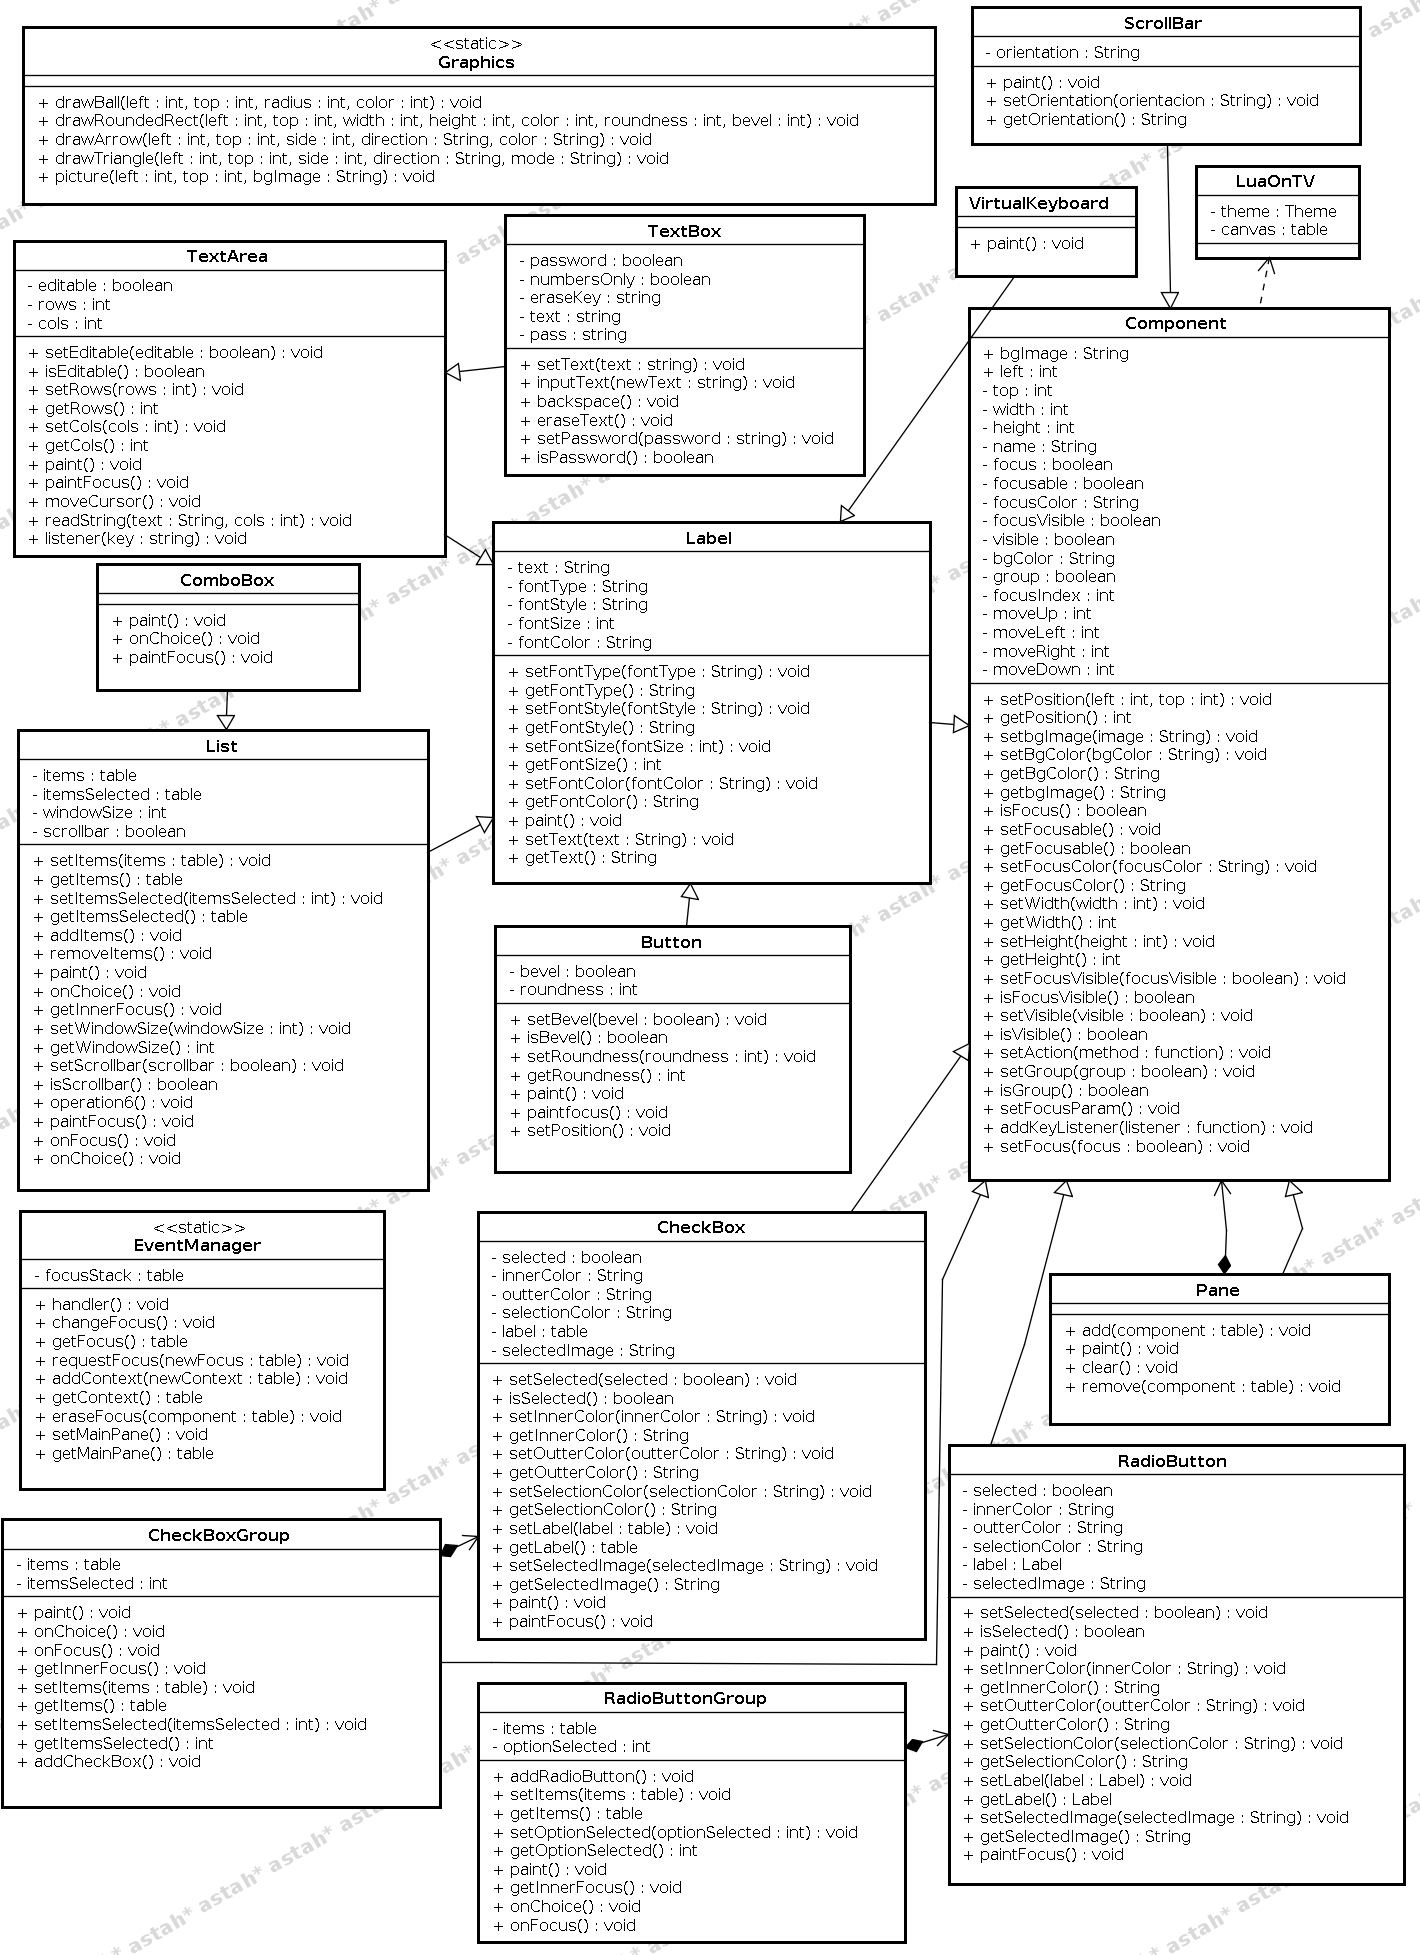
\includegraphics[width=0.6\textwidth]{LuaOnTV-Components.png}
	\label{fig:luaontv-classdiagram}
\end{center}
}

\frame{\frametitle{LuaOnTV 2.0: Máquinas de Estado (EventManager)}
Gráfico de Máquinas de Estados da classe \textit{EventManager}
\begin{center}
	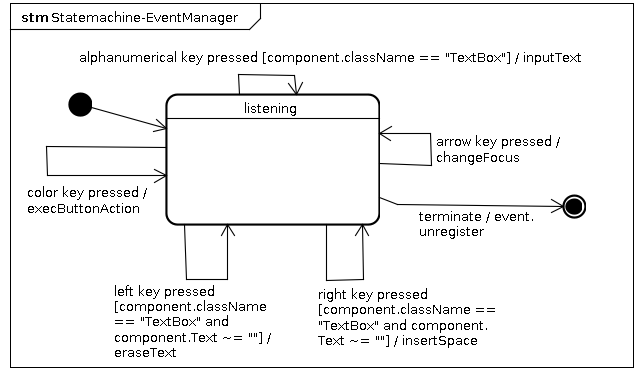
\includegraphics[width=1.00\textwidth]{LuaOnTV-Statemachine-EventManager.png}
	\label{fig:event-manager-statemachine}
\end{center}
}

\frame{\frametitle{LuaOnTV 2.0: Classes de Temas}
Valores padrões das propriedades dos componentes são definidos nas classes e sub-classes de temas
\begin{center}
	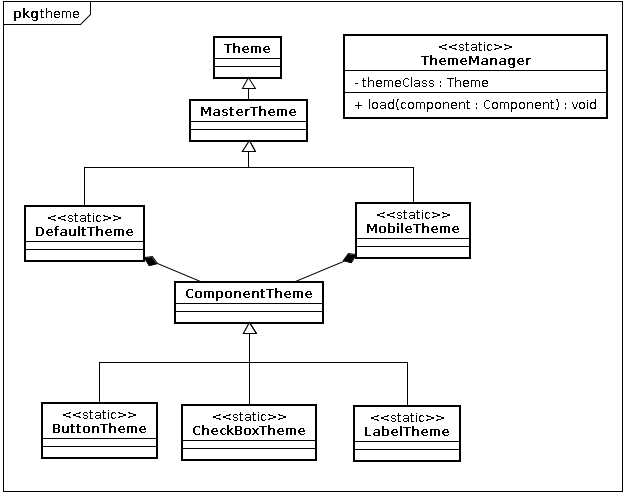
\includegraphics[width=0.8\textwidth]{LuaOnTV-Themes.png}
	\label{fig:luaontv-themes}
\end{center}
}

\frame{\frametitle{LuaOnTV 2.0: Diagrama de Componentes}
\begin{center}
	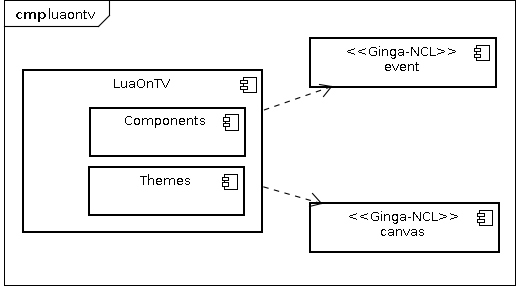
\includegraphics[width=0.7\textwidth]{LuaOnTV-Component-Diagram.png}
  \label{fig:luaontv-component-diagram}
\end{center}
}

\section[Comm]{Framework de Comunicação de Dados}
\frame{\frametitle{Framework de Comunicação de Dados}
\begin{itemize}
	\item Utilizado para a comunicação das diferentes aplicações na arquitetura de T-Commerce proposta;
	\item utilizado para outras aplicações não ligadas a T-Commerce (Web/TV): Cliente de Twitter, Enquete, Quiz, etc;
	\item implementa protocolos HTTP 1.0 e SOAP 1.1 e 1.2;
	\item inexistência de outras implementações (livres) de HTTP e SOAP para o Ginga-NCL.
\end{itemize}
}

\subsection[TCP]{Protocolo TCP no Ginga-NCL}
\frame{\frametitle{Protocolo TCP no Ginga-NCL}
Diagrama de Máquinas de Estados do Módulo \textit{tcp.lua} - Chamadas assíncronas
\begin{center}
	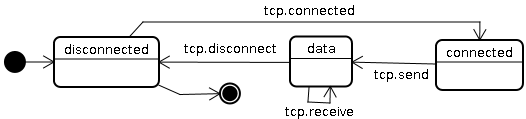
\includegraphics[scale=0.5]{ncluasoap-Statemachine-TCP.png}
	\label{fig:tcp-state-machine}
\end{center}
}

\frame{\frametitle{Protocolo TCP no Ginga-NCL}
Diagrama de Máquinas de Estados do Módulo \textit{tcp.lua} (co-rotinas em execução) - Chamadas assíncronas
\begin{center}
	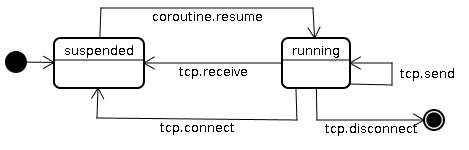
\includegraphics[scale=0.5]{ncluasoap-Statemachine-TCP-Coroutines.png}
	\label{fig:tcp-state-machine-coroutines}
\end{center}

Co-rotinas tornam as chamadas internas (connect, send, receive) síncronas.
}

\subsection[HTTP]{NCLua HTTP}
\frame{\frametitle{NCLua HTTP}
Principais recursos:
\begin{itemize}
  \item implementa HTTP/1.0;
  \item escrito inteiramente em Lua, utiliza o protocolo TCP do Ginga-NCL\cite{abnt200815606};
  \item suporte à autenticação básica, download de arquivos;
  \item suporte à requisições \textit{GET} e \textit{POST};
  \item passagem de parâmetros em requisições \textit{POST};
  \item suporte à passagem de cabeçalhos HTTP;
  \item encapsula todos os detalhes do protocolo TCP do Ginga-NCL.
\end{itemize}

}

\subsection[SOAP]{NCLua SOAP}
\frame{\frametitle{NCLua SOAP}
Principais recursos:
\begin{itemize}
	\item Escrito inteiramente em Lua;
	\item implementa SOAP 1.1 e 1.2;
  \item suporte a parâmetros de entrada e saída do tipo \textit{struct} e \textit{array}; 
  \item facilidade para manipulação de chamadas assíncronas;
  \item simplicidade na obtenção do retorno de uma requisição;
  \item suporte a SOAP \textit{Fault} para captura de erros SOAP;
  \item suporte a SOAP \textit{Header}\cite{soap-spec}.	
\end{itemize}
}

\frame{\frametitle{NCLua SOAP}
Diagrama de Componentes do NCLua SOAP e NCLua HTTP
\begin{center}
	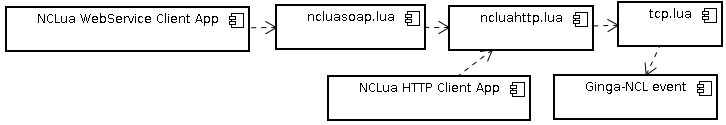
\includegraphics[width=0.8\textwidth]{ncluasoap-component-diagram.png}
	\label{fig:diagrama-componentes}
\end{center}
}

\subsection[Apps]{Algumas aplicações desenvolvidas com o Framework}
\frame{\frametitle{Algumas aplicações desenvolvidas com o Framework}
\begin{itemize} 
	\item \textbf{Enquete TVD}: enquete com registro de voto e apuração a partir de servidor \textit{Web};
  \item \textbf{NCLua RSS Reader}: leitor de notícias RSS de um provedor de conteúdo na \textit{Web};
  \item \textbf{NCLua Tweet}: envio e recebimento de mensagens pelo micro \textit{blog Twitter};
  \item \textbf{TVD Quiz}: Aplicação de perguntas e respostas para TVD.
\end{itemize}
}


\subsection[Avaliação]{Avaliação de Desempenho do NCLua SOAP}
\frame{\frametitle{Avaliação de Desempenho do NCLua SOAP}
A Tabela a seguir apresenta os resultados de avaliações de desempenho para algumas das aplicações testadas.

\begin{center}
\scriptsize{
	\begin{tabular}{|p{3.5cm}|p{1.8cm}|p{1.8cm}|p{1cm}|p{1cm}|} %{|l|c|c|}
  \hline
		\textbf{\textit{Web Service} consumido} & 
		\textbf{Parâmetros} \par\textbf{de entrada} &
		\textbf{Geração req:}\par\textbf{método \textit{call}} \textbf{(seg)} & 
		\textbf{RAM}\par\textbf{(KB)} &
		\textbf{\% CPU}\\
  \hline
		Situação do tempo\par \url{http://www.deeptraining.com/webservices/weather.asmx} & 
		\textit{City} = "Brasília" & 0.13 & 121.78 & 0.3 \\
  \hline
		Conversão de Moeda\par
		\url{http://www.webservicex.net/CurrencyConvertor.asmx} &
		\textit{FromCurrency} = "USD"\par        
    \textit{ToCurrency} = "BRL" & 
    0.13 & 121.65 & 0.3 \\  
  \hline
		Consulta de endereço a partir do CEP\par
		\url{http://www.maniezo.com.br/webservice/soap-server.php} &
    cep = "77021682" & 
    0.13 & 133.17 & 0.3 \\  
	\hline
	\end{tabular}
	\captionof{Avaliação de Desempenho do NCLua SOAP}
	\label{tab:analise-desempenho}
}
\end{center}
}

\frame{\frametitle{Comparativo entre o NCLua SOAP e outros toolkits SOAP}
A Tabela a seguir apresenta um comparativo entre alguns \textit{toolkits} SOAP
e o NCLua SOAP.
\begin{center}
\scriptsize{
	\begin{tabular}{|p{4cm}|p{0.7cm}|p{0.9cm}|p{0.7cm}|p{1.2cm}|p{1.2cm}|} %{|l|c|c|}
  \hline
		\textbf{Características} & 
		\textbf{Axis} &
		\textbf{Axis2} &		
		\textbf{PHP} &		
		\textbf{gSOAP} &		
		\textbf{NCLua SOAP} 
    \\
  \hline
		Linguagem & Java & Java & PHP 5 & C++ & NCLua \\  
  \hline
		SOAP 1.1 & Sim & Sim & Sim & Sim & Sim \\  
  \hline
		SOAP 1.2 & Sim & Sim & Sim & Sim & Sim \\  
  \hline
		SOAP com Anexos & Sim & Sim & Sim & Sim & Ainda não \\  
  \hline
		Geração de código cliente a partir do WSDL & Sim & Sim & Sim & Sim & Ainda não \\  
  \hline
		Suporte para formato \textit{document/literal} & Bom & Bom & Médio & Bom & Bom \\  
  \hline
		Requisitos de \textit{runtime} & JVM & JVM & PHP engine & Nenhum & Ginga-NCL \\  
  \hline
		Documentação & Boa & Pequena & Média & Boa & Média \\  		
	\hline
	\end{tabular}
	\captionof{Comparação entre NCLua SOAP e outros \textit{toolkits} SOAP (adapt. \cite{louridas2006soap}).}
	\label{tab:comparacao-toolkits-soap}
}
\end{center}
}


\subsection[Comparativo]{Comparativo entre módulos desenvolvidos e o tcp.lua}
\frame{\frametitle{Comparativo entre módulos desenvolvidos e o tcp.lua}
A tabela a seguir mostra como a quantidade de código é reduzida com o uso dos módulos implementados,
que compõem o Framework de Comunicação de Dados.
\begin{center}
\scriptsize{
	\begin{tabular}{|p{2cm}|p{4cm}|p{4cm}|} %{|l|c|c|}
  \hline
		\textbf{Aplicação / Protocolo} & \textbf{Sem módulos implementados} & \textbf{Com módulos implementados} \\
  \hline
		Enquete/HTTP & 14 linhas de código\par5 funções utilizadas diretamente & 
    5 linhas de código = 35\% do anterior\par1 função usada diretamente \\
  \hline
		Cotação do dólar/SOAP & 64 linhas de código\par5 funções utilizadas diretamente & 
    15 linhas de código = 23\% do anterior
    \par(9 são parâmetros do WS) 1 função usada diretamente \\
  \hline
	\end{tabular}
	\captionof{Comparativo entre aplicações de TVD com e sem os módulos implementados}
	\label{tab:comparativo-propostas}
}
\end{center}
}

\section{Publicações}
\frame{\frametitle{Publicações}
\begin{itemize}
	\item de Castro Monteiro, C., Pereira, H. C., da Silva Filho,
M. C., de Lira Gondim, P. R., and de Miranda Rios, V. (2010). Implementacao de um
Set-top Box Virtual para Desenvolvimento e Testes de Aplicacoes para TV Digital Interativa. 
\textit{International Information and Telecommunication and Technologies Conference} (I2TS 2010). Florianópolis, SC.
  \item da Silva Filho, M. C., de Lira Gondim, P. R. NCLua SOAP: Acesso a \textit{Web Services} em aplicações de TVDi. 
  Simpósio Brasileiro de Sistemas Multimídia e Web (WebMedia 2011). Florianópolis, SC. (aguardando avaliação)
  \item da Silva Filho, M. C., de Lira Gondim, P. R. 
  Integração entre Web e TV com NCLua HTTP e NCLua SOAP. \textit{Journal of Brazilian Computer Science} (JBCS) (a ser submetido)
\end{itemize}
}


\section{Conclusões}
\frame{\frametitle{Conclusões}
\begin{itemize}
	\item Requisitos levantados foram todos atendidos;
	\item arquitetura proposta serve de base para o desenvolvimento de serviços de \textit{T-Commerce} para o SBTVD;
	\item implementações dos protocolos HTTP e SOAP mostraram como a solução proposta
é eficiente em uso de processador e RAM, sendo uma solução ideal para equipamentos como \textit{Set-top Boxes};
  \item os protocolos implementados são a base da integração entre \textit{Web} e TV
e estão sendo bastante úteis em outros trabalhos;
  \item a implementação de SOAP foi ganhadora do 1o. Concurso latino-americano de conteúdo para TV Digital Interativa;
  \item \textit{framework} LuaOnTV permite a construção de GUI's com suporte a múltiplos dispositivos,
  possibilitando ter uma única aplicação para TV, Celular e Notebook.
\end{itemize}
}


\section{Referências Bibliográficas}
\begin{frame}[allowframebreaks]  
  \frametitle{Referências Bibliográficas}
  \bibliographystyle{sbc} 
  \bibliography{../dissertacao/referencias,../dissertacao/referencias-artigo}
\end{frame}


%\lstinputlisting[language=TeX, label=exemplo1, caption={``Olá mundo em LaTeX''}]{ola_mundo.tex}

\end{document}
